\documentclass[11pt]{report}
\usepackage{amsmath}
\usepackage{sectsty}
\linespread{1.1}
\usepackage
[
a4paper,% other options: a3paper, a5paper, etc
left=3cm,
right=3cm,
top=3cm,
bottom=4cm,
% use vmargin=2cm to make vertical margins equal to 2cm.
% us  hmargin=3cm to make horizontal margins equal to 3cm.
% use margin=3cm to make \textsl{}all margins  equal to 3cm.
]
{geometry}
\usepackage{titlesec}
\titleformat{\chapter}[display]
{\normalfont\bfseries}{}{0pt}{\Large}
\titleformat*{\section}{\normalsize\bfseries}
\usepackage{etoolbox}
\makeatletter
\patchcmd{\chapter}{\if@openright\cleardoublepage\else\clearpage\fi}{}{}{}
\makeatother
\usepackage{graphicx}
\graphicspath{ {C:/Users/sai/MathLaTeXstuff/semprojsem5/} }
\usepackage{amssymb}
\usepackage[medium]{titlesec}
\usepackage{amsfonts}
\let\emptyset\varnothing
\usepackage{amsthm}
\usepackage{amsopn}
\usepackage{bbm}
\usepackage{thmtools}
\declaretheoremstyle[notefont=\bfseries,notebraces={}{},%
headpunct={},postheadspace=1em]{mystyle}
\declaretheorem[style=mystyle,numbered=no,name=Theorem]{thm-hand}
\theoremstyle{plain}
\newtheorem{thm}{Theorem}[chapter] % reset theorem numbering for each chapter
\sectionfont{\fontsize{12.5}{15}\selectfont}
\theoremstyle{definition}
\newtheorem{defn}{Definition}
\newtheorem{cnjc}{Conjecture}
\newtheorem{exmp}{Example} % same for example numbers
\usepackage[utf8]{inputenc}
\usepackage[english]{babel}
\newcommand{\lnorm}[1]{\left\|}
\newcommand{\rnorm}[1]{\right\|}
\renewcommand\qedsymbol{$\blacksquare$}
\newtheorem{theorem}{Theorem}
\newtheorem{lemma}[theorem]{Lemma}
\newtheorem{coro}{Corollary}
\newcommand\inner[2]{\langle #1, #2 \rangle}
\usepackage{kantlipsum,graphicx}
\begin{document}
	\begin{titlepage}
		\centering
		\vspace*{0.6in}
		\bgroup
		\hrule
		\vspace{0.2in}
		\huge \textbf{On Quaternions and Octonions} 
		\vspace{0.2in}
		\hrule
		\egroup
		\vspace{0.5in}
		\bgroup
		\Large Sujeet Bhalerao\\[0.1in]
		\egroup
		20151115\\
		\vspace{0.5in}
		MTH301 
		\vspace{0.7in}
		\vspace{0.6in}
				
		Project supervisor:\\[0.2in]
		\Large Dr. Steven Spallone 
		\par
		\vspace{0.5in}
		
		\par
		\vspace{0.1in}
		
		\vspace{0.2in}
		\vfill
		\today
	\end{titlepage}

\chapter{Quaternions and geometry}

Quaternions (denoted by $ \mathbb{H} $) are usually represented in the form $  a + bi + cj + dk $ where $ a, b, c, d $ $ \in \mathbb{R}$ and $ i, j, k $ satisfy  $  i^2 = j^2 = k^2 = ijk = -1 $. They  can be represented as pairs of complex numbers (which themselves can be thought of as pairs of real numbers). The Cayley-Dickson construction uses this representation extensively. The quaternion $ a + bi + cj + dk $ corresponds to the complex pair $ (a+ib, c+id) $.
\begin{exmp}
Multiplication of quaternions is not commutative: $ ij = k \neq ji = -k $.
\end{exmp}
 \noindent As a vector space over $ \mathbb{R} $, $ \mathbb{H} $ is isomorphic to $ \mathbb{R}^4 $. The map $ a+ib+jc+dk \mapsto (a,b,c,d) $ is an isomorphism between the two vector spaces.

\section{$ O_n $ and $ GO_n $}
\begin{defn}
	A linear map $ L: $ $ \mathbb{R}^n  \rightarrow  \mathbb{R}^n$ is said to be  \textbf{orthogonal }(or a \textbf{Euclidean congruence}) if  $ \|Lv\| = \|v\| $ for all $ v \in \mathbb{R}^n. $
\end{defn}
	\begin{exmp}
	As an example, consider the linear map $ L : \mathbb{R}^2 \to \mathbb{R}^2 $ given by $ L(x,y)=(y,x) $. The matrix representation of $ L $ w.r.t the standard basis is 
	$$ L = \begin{pmatrix}
	0 & 1\\
	1 & 0
	\end{pmatrix}. $$\\
	Let $ v $ = $ \begin{pmatrix}
	x \\
	y 
	\end{pmatrix} $ be an arbitrary element of $ \mathbb{R}^2 $. We now verify that $ L $ satisfies the condition for being orthogonal, that is, $ \left\|Lv\right\| = \left\| v\right\|.  $
	\\
	\vspace{2mm}
	
	$$ \|Lv\| = \left\| \begin{pmatrix}
	0 & 1\\
	1 & 0
	\end{pmatrix}\begin{pmatrix}
	x \\
	y 
	\end{pmatrix}\right\|  = \left\| \begin{pmatrix}
	y \\
	x 
	\end{pmatrix}\right\|  = \|v\|.$$\vspace{2mm} \\ 
	
	Therefore $  L $ is orthogonal.
	
	\end{exmp}
	
\begin{defn}
	A linear map $ L: $   $\mathbb{R}^n  \rightarrow  \mathbb{R}^n$ is a \textbf{Euclidean similarity} if there exists $\lambda \in  \mathbb{R}_{>0} $ such that  $ \|Lv\|
	= \lambda \|v\| $ for all $ v $ $ \in  \mathbb{R}^n. $ Then, $ \lambda $	is called the multiplier.
\end{defn}
 \begin{exmp}
 	We claim that the following matrix $ L $ is an example of a Euclidean similarity of $ \mathbb{R}^2 $
 \end{exmp}
 $$ 
L=
\begin{pmatrix}
0 & 2\\
-2 & 0
\end{pmatrix}$$
Let $ v  $
 be any element of $ \mathbb{R}^2. $ Written as a column vector, we have
$$ v =  \begin{pmatrix}
x\\
y
\end{pmatrix} $$
\ \\ \\
Then , $ \|v\| = \sqrt{x^2 + y^2} $.\\ \\ We now check that there does indeed exist a multiplier $ \lambda $ such that $ \left\| Lv\right\| =\lambda\left\| v\right\| $ . \vspace{4mm}

$$ \left\| Lv\right\|   =  \left\| \begin{pmatrix}
0 & 2\\
-2 & 0
\end{pmatrix}  \begin{pmatrix}
x\\
y
\end{pmatrix} \right\|   = \left\| \begin{pmatrix}
2x\\
-2y
\end{pmatrix}\right\|  =   2 \sqrt{x^2+y^2} =  2 \|v\|. $$ \vspace{4mm}\\		
  Therefore, $\text{$ L $ is a Euclidean similarity of $ \mathbb{R}^2 $ with }  \lambda = 2 $. \\

\begin{lemma}
	The following holds for all $ v,w $ belonging to a inner product space V over $ \mathbb{R}$ :
	$$ \inner{v}{w} = \dfrac{\|v + w\|^2 - \|v - w\|^2}{4}$$ 
\end{lemma}
\begin{proof}
	We use the fact that norms and inner products are related by $ \inner{v}{v} = \|v\| ^2 $ to rewrite the right side of the required identity as 
\begin{align*}
	& \dfrac{\|v + w\|^2 - \|v - w\|^2}{4}\\ \\ &= \dfrac{\inner{v+w}{v+w} - \inner{v-w}{v-w}}{4}\\ \\ 
	  &=\dfrac{\inner{v}{v} + 2\inner{v}{w} + \inner{w}{w} - (\inner{v}{v} - 2\inner{v}{w} + \inner{w}{w})}{4}\\ \\
	   &= \inner{v}{w}. 
\end{align*}
\end{proof}

\begin{theorem}
	If a linear map	$ L $:   $\mathbb{R}^n  \rightarrow  \mathbb{R}^n$ is a Euclidean similarity with multiplier $ \lambda $, then\\ $\inner{Lv}{Lw}= \lambda^2 \inner{v}{w} .$
\end{theorem}
\begin{proof}
	By Lemma 1, we can write
	\begin{align*} 
	 \inner{Lv}{Lw} &=  \dfrac{\|Lv + Lw\|^2 - \|Lv - Lw\|^2}{4} \\ \\ 
	 &=  \dfrac{\|L(v + w)\|^2 - \|L(v - w)\|^2}{4}\\ \\
	 &= \dfrac{\|\lambda(v + w)\|^2 - \|\lambda(v - w)\|^2}{4}\\ \\
	 &= \dfrac{\lambda^2(\|(v + w)\|^2 - \|(v - w)\|^2)}{4}\\ \\
	 &= \lambda^2 \inner{v}{w} .
	\end{align*}
	 
	
\end{proof}


\begin{defn}
	The \textbf{orthogonal group $ O_n $} is the group of Euclidean congruences of $ \mathbb{R}^n $. Equivalently, it is the group of $ n \times n  $ orthogonal matrices. A proof of this equivalence is given in Theorem 4. \\
\end{defn}	
\begin{defn}
	The \textbf{general orthogonal group} $ GO_n $ is the group of Euclidean similarities of $ \mathbb{R}^n $.\\
\end{defn}

\begin{theorem}
	The map $ L \mapsto \lambda $ which sends each similarity of $ \mathbb{R}^n $ to its multiplier is a homomorphism from $ GO_n $ to $ \mathbb{R}_{>0} $. The kernel of this map is $ O_n $.\\
\end{theorem}
	\begin{proof}
		For the given map to be a homomorphism, it must send the composition of two similarities $ L_1 $ and $ L_2 $ to the product of their multipliers $ \lambda_1 $ and $ \lambda_2 $. To put it slightly differently, the similarity $ L_1 \circ L_2 $ must have multiplier $ \lambda_1 \lambda_2 $. This is true because one can write $ \left\| L_1\circ L_2(v)\right\| = \left\| L_1(L_2(v))\right\| = \lambda_1\left\|L_2(v) \right\| = \lambda_1 \lambda_2 \left\|v \right\|.   $\\
		 
		The kernel of the given map is the set containing all elements of $ GO_n $ which have multiplier $ 1 $. Therefore, $ \left\|Lv \right\|  = \left\|v \right\| ,\forall v \in \mathbb{R}^n$ is true for each element $ L $ in the kernel. This implies that the kernel is the collection of Euclidean congruences of $ \mathbb{R}^n $ which is precisely $ O_n $.
		
	\end{proof}






\begin{defn}
	If $ W $ is a subspace of a vector space $ V$, the codimension of $ W $ is defined as 
	$$\text{codim  $ W $ = dim  $ V $ $ - $ dim  $ W $}  $$ $ W $ is said to be a \textbf{hyperplane} in $ V $ if  \text{codim} $ W $ = 1.
\end{defn}

 \begin{exmp}
	Lines and planes are hyperplanes in $ \mathbb{R}^2 \text{ and } \mathbb{R}^3 $ respectively.
 \end{exmp}

\begin{theorem}
	Let $ A $ : $ \mathbb{R}^n \rightarrow \mathbb{R}^n$ be a linear transformation. The following are equivalent:\\	$ 1) AA^T=I.$ \\2) For all $  v \in  \mathbb{R}^n $ $ \|Av\|	= \|v\| $. \\3) For all $  v,w \in  \mathbb{R}^n , \inner{Av}{Aw} = \inner{v}{w}  $.
\end{theorem}
\begin{proof}We first prove that statements 2 and 3 are equivalent. Then we show that 1 $ \Longrightarrow $ 2 \text{ and } 3 $ \Longrightarrow $ 1.\\
\\We start by proving $ 3 \Longrightarrow 2 $.\\
From (3) we have, 
\begin{align*}
 \inner{Av}{Aw} &= \inner{v}{w} \quad \forall v,w \in \mathbb{R}^n . \\
 v = w &\implies
\inner{Av}{Av} = \inner{v}{v}.\\ 
&\implies \|Av\|=\|v\|.
\end{align*}
  
 \text{To show the converse, we use Lemma 1 to write}  


\begin{align*}
\inner{Av}{Aw} &= \dfrac{\|Av + Aw\|^2 - \|Av - Aw\|^2}{4}\\ \\
 &= \dfrac{\|A(v+w)\|^2 - \|A(v-w)\|^2}{4}\\ \\ 
&= \dfrac{\|v + w\|^2 - \|v - w\|^2}{4}\\ \\ 
&= \inner{v}{w}.
\end{align*}


Now we show $ 1 \Longrightarrow 2 $.
\begin{align*}
\|Av\| &= \sqrt{\inner{Av}{Av}}\\
&= \sqrt{Av.Av}\\
&= \sqrt{(Av)^\intercal (Av)}  \\ 
&=\sqrt{v^\intercal A^\intercal A v} \\
&= \sqrt{v^\intercal v}\\
&= \|v\|.
\end{align*}

	
		
The proof is completed by showing $ 3 \Longrightarrow 1. $

$3 \Longrightarrow  \inner{Av}{Aw} = \inner{v}{w}$ \: $\forall v,w \in \mathbb{R}^n$.
\begin{align*}
\inner{Av}{Aw} &= Av.Aw\\ 
&= (Av)^\intercal (Aw)\\
&= v^\intercal A^\intercal A w\\
&= v^\intercal  w.\\ 
\text{ It suffices to show that if } v^\intercal B w &= v^\intercal B' w \: \forall v, w \in \mathbb{R}^n, \text{then } B = B'. \text{ This implies }AA^\intercal = I.	
\end{align*}

Since $ v^\intercal B w = v^\intercal B' w $ is true for all $ v, w \in \mathbb{R}^n $,

$ (e_i)^\intercal B e_j = (e_i)^\intercal B' e_j. \text{ This gives } b_{ij} = b'_{ij}. \text{ Hence}, B = B'.
 $


\end{proof}
\begin{theorem}
	All eigenvalues $ \lambda $ of an orthogonal matrix $ A $ satisfy $ |\lambda| = 1. $ 
\end{theorem}
\begin{proof}
	Any eigenvalue $ \lambda $ must satisfy $ Av = \lambda v. $ Since $ A $ is an orthogonal matrix, we must have $ \|Av\| = \|v\|. $ Therefore $ \|\lambda v \| = \|v\| $. Since $ \|v\|$ is nonzero,  $ |\lambda| = 1. $
\end{proof}
\begin{theorem}
	If $ L  \in  GO_n $ with $L( v $) = $ v $, then $L(v^\bot$) = $v^\bot$.\\
	Here, $v^\bot$ = $\{w \in V : \inner{v}{w} = 0\}.  $ 
\end{theorem}
\begin{proof}
	We show set inclusion both ways.\\
	Suppose $ w $ $ \in v^\bot $. Then $ \inner{v}{L(w)}= \inner{L(v)}{L(w)}=\lambda^2\inner{v}{w} = 0 $. Therefore, $ L(v^\bot)\subset v^\bot.$ \\To show the reverse inclusion, let $ w \in v^\bot $. We must show that $ w = L(u)$ for some  $u \in v^\bot .$ Observe that $ u = L^{-1}(w) \in v^\bot $ since $ \inner{v}{L^{-1}(w)} = \inner{L^{-1}(v)}{L^{-1}(w)} = \lambda^2\inner{v}{w} = 0. $
\end{proof}
\section{Quaternions and 3-dimensional rotations}
\begin{theorem}
	There exists a linear map $ L : \mathbb{R}^3 \to \mathbb{R}^3 $ given by $ L(v)=qvq^{-1} $ where $ q $ is a quaternion of the form $ ai+bj+ck. $ Moreover, $ L $ is a Euclidean congruence of $ \mathbb{R}^3 $.	
\end{theorem}
\begin{proof}
	Consider the linear map $ L: $   $\mathbb{R}^4  \to  \mathbb{R}^4$ given by $ L(v)=q_1 v q_2 $ where $ q_1 \text{ and } q_2 $ are quaternions. Recall that $ \mathbb{H}  $ and $ \mathbb{R}^4 $ are isomorphic. Each element $ (a,b,c,d) \text{ of } \mathbb{R}^4 $ can thus be identified with the quaternion $  a+bi+cj+dk. $  We have, $ N(q_1vq_2) = N(q_1)N(v)N(q_2) $ where $ N(a+ib+cj+dk)=a^2+b^2+c^2+d^2 $.  $ \text{Therefore, }L $ $ \in GO_4$ with multiplier $\lambda =  \sqrt{N(q_1)N(q_2)}. $\ If $ L(\mathbbm{1})=\mathbbm{1} $, by Theorem 5, $ L $ must fix the 3-dimensional space perpendicular to $ \mathbbm{1} $, which contains elements of the form $ ai + bj + ck $ (since the inner product with $ \mathbbm{1} $ must be 0). $ L $ fixes $ \mathbbm{1} $ if $ q_2 = q_1^{-1} $. $ \text{Hence, }$ $ L(v)=qvq^{-1}$ fixes a 3-dimensional space perpendicular to $ \mathbbm{1} $, which is isomorphic to $\mathbb{R}^3.$ Also, $ L \in O_3 $ because $ N(qvq^{-1})=N(v). $ 
\end{proof}
\section{Reflections in $\mathbb{R}^n$}
\begin{lemma}
	Suppose $ v $ is a nonzero element of $ \mathbb{R}^n $. Let $ H = v^\bot $. So $ \mathbb{R}^n = \mathbb{R}v \oplus H.$ Every element $ w $ of $ \mathbb{R}^n $ can be written uniquely in the form $ w = \lambda v + h $, with $ \lambda \in \mathbb{R} $, $ h\in H $. 
\end{lemma}
\begin{defn}
	The reflection $ s_v $ of $ \mathbb{R}^n $ determined by $ v $ is defined as $ s_v (w) = (-\lambda)v + h$, for $ w $ as in Lemma 8. 
\end{defn}
\begin{exmp}
Pick $$ v = e_2 = \begin{pmatrix}
0 \\
1 \\
0 
\end{pmatrix} \in \mathbb{R}^3.$$ Since $ e_1 $ and $ e_2 $ belong to $ v^\bot $, the matrix form of $ s_{e_2}  $ is 
$$ \begin{pmatrix}
1 & 0 & 0\\
0 & -1 & 0 \\
0 & 0 & 1\\
\end{pmatrix} $$.\\	
\end{exmp} 
We now prove a few theorems about reflections.
\begin{theorem}
	The eigenvalues of a reflection are $ \pm $ 1.
\end{theorem} 
	\begin{proof}
		For any eigenvalue $ \beta $ and eigenvector $ w = \lambda v + h $ of $ s_v $ we must have $ s_v (w) = \beta w $ , i.e., $-\lambda v + h = \beta \lambda v + \beta h $ . Rearranging this equation and using the fact that $ v $ and $ h $ are perpendicular gives us the desired result.
	\end{proof}
	\begin{theorem}
 The $ -1 $ eigenspace is $ \mathbb{R}v, $ and $ +1 $ eigenspace is $ H $.

	\end{theorem}
	\begin{proof}
		The elements of the $ -1 $ eigenspace must satisfy $ s_v (w) = -w  $. Therefore, we have $ -\lambda v + h = -\lambda v - h  $ which gives $ h =0. $ $ w $ is thus of the form  $ \lambda v $ which clearly lies in $ \mathbb{R}v.$\\
		Similarly, the elements of the $ +1 $ eigenspace satisfy $ s_v (w) = w  $, which gives $ \lambda =0 $ and thus $ w = h $, for some $ h $ in $ H $. Hence $ H $ is the +1 eigenspace.
	\end{proof}
	\begin{theorem}
 For any reflection $ s_v ,$ $ s_v ^2 = \mathbbm{1}. $
	\end{theorem}
	\begin{proof}
		Suppose $ w = \lambda v + h $ for some $ \lambda \in \mathbb{R} $ and $ h \in v^\bot $. Then $ s_v ^2 (w) = s_v(s_v(\lambda v + h )) = s_v(-\lambda v + h) = (\lambda v + h) = w. $
	\end{proof}
	\begin{theorem}
		Reflections are orthogonal.
	\end{theorem}
	\begin{proof}
		We use Theorem 4 to show they preserve inner products and hence are orthogonal.
		We have 
	\begin{align*}
		 \inner{s_v(w_1)}{s_v(w_2)} &= \inner{-\lambda_1 v_1+h_1}{-\lambda_2 v_2+h_2}\\ \\ 
		&= \inner{-\lambda_1 v_1+h_1}{-\lambda_2 v_2+h_2}\\ \\ 
		&= \lambda^2 \inner{v_1}{v_2} + (-\lambda) \inner{v_1}{h_2} + (-\lambda) \inner{h_1}{v_2} +\inner{h_1}{h_2}\\ \\
		&= \lambda^2 \inner{v_1}{v_2} + \inner{h_1}{h_2}\\ \\ 
		&= \inner{w_1}{w_2}.  
	\end{align*}
		We use the fact that $ v_1 $ and $ v_2 $ are perpendicular to $ h_2 $ and $ h_1 $ respectively.
	\end{proof}
	

\chapter{Quaternions and number theory}
\section{Euclidean algorithm for rational integers}
We begin by recalling the Euclidean algorithm for rational integers before moving on to the Gaussian integers. Throughout this section, the word `integer' denotes a rational integer. \\ 
The Euclidean algorithm is a method for computing the gcd of two numbers $ a $ and $ b $. The division algorithm states that given any two integers $ a $ and nonzero $ b $ with $ a > b $, there exist unique integers $ q $ and $ r $ such that $  a=bq+r $ such that $ 0 \leq r < b.  $
If the remainder $ r $ obtained using the division algorithm is non-zero, we apply the division algorithm to $ b $ and $ r $ to get
$$ b=rq_1 + r_1 \text{ with } 0 \leq r_1 < r. $$

This process can be repeated with $ r $ and $ r_1 $, $r_1$ and $ r_2 $ and so on until one obtains, for some $ n ,$ $ r_{n+1}=0 $. This will eventually occur because $ r_1, r_2, r_3 ... $ is a strictly decreasing sequence of integers bounded below by zero. The last steps of the algorithm will look like:
\begin{align*}
& \vdots \\
r_{n-2} =& \,r_{n-1} q_n + r_n \\
r_{n-1} =& \,r_n q_{n+1} + 0 . \\
\end{align*}

\begin{lemma}
	Let $ a, b, q ,r \in \mathbb{Z}$ such that $ a = bq + r. $ Then $ \gcd(a,b) = \gcd(b,r) $.
\end{lemma}
\begin{proof}
	We show that $ \gcd(a,b) $ and $ \gcd(b,r)$ are divisors of each other.\\
	By definition of gcd, we have that $ \gcd(a,b) \mid a,\,  \gcd(a,b) \mid b$. Therefore, $ \gcd(a,b) \mid r.$ By the definition of gcd (again), we have $  \gcd(a,b) \mid  \gcd(b,r).  $ Nearly identical reasoning gives us $  \gcd(b,r) \mid  \gcd(a,b).  $ Thus we have $ \gcd(a,b) = \gcd(b,r) $.
\end{proof}
\textbf{Claim.} $ \gcd(a,b) = r_n .$ 
\begin{proof}
	  By Lemma 13, we have that $ \gcd(a,b) = \gcd(b,r) = \gcd(r,r_1) = ... = \gcd(r_{n-1},r_n) = \gcd(r_n,0) = r_n. $
\end{proof}
We state a few definitions to get started on the general notion of an `integer'. 
\begin{defn}
	A \textbf{Gaussian integer} is a complex number of the form $ a + bi $ where $ a $ and $ b $ are rational integers. 
\end{defn}
\begin{defn}
	An \textbf{Eisenstein integer} is a complex number of the form $ a + b \omega $ where $ a $ and $ b $ are rational integers and $ w  = \frac{-1 + i \sqrt{3}}{2}$.  
\end{defn}
\begin{defn}
	A \textbf{Kleinian integer} is a complex number of the form $ a + b\lambda $ where $ a $ and $ b $ are rational integers and $ \lambda = \frac{-1+i\sqrt{7}}{2}$.
\end{defn}
\begin{defn}
	A \textbf{Hurwitz integer} is a quaternion of the form $ a + bi + cj + dk $ where $ a,b,c,d $ are all rational integers or all multiples of $ \frac{1}{2} $ .
\end{defn}
\begin{defn}
	A \textbf{Lipschitz integer} is a quaternion of the form $ a + bi + cj + dk $ where $ a,b,c,d $ are all rational integers.
\end{defn}
\section{Gaussian integers}
The Gaussian integers are denoted by $ \mathbb{Z}[i]. $\\
A few pertinent definitions from ring theory are stated before we study $ \mathbb{Z}[i]. $\\
Let $ R $ be a commutative ring.
\begin{defn}
		 An element $ x \text{ of } R  $ is said to be a \textbf{unit}  if there exists a $ y \in R $ such that $ xy = 1_R. $
\end{defn}
\begin{defn}
		Two elements $ x , y \in R $ are said to be \textbf{associates} if there exists a unit $ u $ such that $ x = uy $. 
\end{defn}

\begin{defn}
	A nonzero element $ x \in R $ is said to be \textbf{irreducible} if $ x = yz \text{implies }y \text { or } z $ is a unit.
\end{defn}
\begin{defn}
		A nonzero element $ x \in R $ is said to be \textbf{prime} if $ x $ is not a unit and $ x \mid yz \implies x\mid y \text { or } x \mid z $.
\end{defn}
	Primes and irreducibles in a ring are not always the same. 

	\begin{exmp}
	Consider the ring $ \mathbb{Z}[\sqrt{-5}]$. We show that $3  \in \mathbb{Z}[\sqrt{-5}] $ is irreducible but not prime. $ 3\mid(2+\sqrt{-5})(2-\sqrt{-5}) $ but it does not divide either of the two factors. Therefore 3 is not prime. We show $ 3 $ is irreducible: suppose $ 3 = pq. $ Then applying norm gives us $ 9 = N(p)N(q). $ Since $ N(a+b\sqrt{-5}) = a^2 + 5b^2 = 3$ has no solutions, one of $ p $ or $ q $ must be a unit.

	\end{exmp}

\begin{defn}
	The norm of a Gaussian integer $ a+bi $ is defined as $ N(a+bi) = a^2 + b^2.$
\end{defn}
It is clear that the norm of any nonzero Gaussian integer is a positive integer.
\begin{theorem}
	The following statements are equivalent: \\ 
	1) $ u \in \mathbb{Z}[i]$ is a unit.\\
	2) $N(u) = 1. $	 
\end{theorem}
\begin{proof}
	Suppose $ u \in \mathbb{Z}[i] $  is a unit. Therefore, there exists $ y \in \mathbb{Z}[i] $ such that $ uy = 1. $ Hence $ N(uy)=1. $ By multiplicativity of norm, $ N(u)N(y)=1. $ Since each of $ N(u) \text{ and }N(y) $ are positive integers, we must have $ N(y)=N(u)=1. $\\
	Conversely, suppose that $ N(u)=1 $. By definition of norm, $ u\bar{u}=1 $. Since $\bar{u} \in  \mathbb{Z}[i] $, $ u $ is a unit.
\end{proof}
\begin{theorem}
	There are four units in the Gaussian integers, namely $ 1,\, -1,\, i,\, -i.$
\end{theorem}
\begin{proof}
	By Theorem $ 14 $, every unit has norm $ 1 $. If $ u = a+bi $ is a unit, $ a^2 + b^2 = 1 $. The number of solutions $ (a,b) $ to this equation are precisely four: $ (1,0),\,(0,1),\,(-1,0),\,(0,-1). $ These correspond to $ 1,\, -1,\, i,\, -i.$
\end{proof}
\begin{theorem}
		The division algorithm for Gaussian integers states that if $ Z $ and $ z $ are two Gaussian integers, then there are Gaussian integers $ Q $ and $ R $ such that $ N(R)<N(z) $ and $ Z=zQ+R $.
		\begin{proof}
			Let $ Zz^{-1} = x + yi$. Define $ Q = X + Yi $ to be the closest Gaussian integer to $ x+yi $ and $ R = Z-zQ $. We will thus have $ |X-x|\leq 1/2 $ and $ |Y-y|\leq 1/2 $. It remains to show that $ N(R)<N(z) $. Observe that $ N(Rz^{-1}) = N(Zz^{-1}-Q) = (x-X)^2+(y-Y)^2 \leq \frac{1}{4} + \frac{1}{4} = \frac{1}{2}. $
			Therefore $ N(R)\leq \frac{1}{2} N(z) $. This completes the proof.
			
		\end{proof}
	Note that the Gaussian integers $ Q $ and $ R $ obtained in the division algorithm need not be unique.
	\begin{exmp}
 For example, if we have $ Z = 3+3i$ and $z = 2+0i,$ we can write $ 3+3i = 2(2+2i) + (-1-i) $ and $ 3+3i = 2(1+i)+(1+i) $. In each case we have $ N(-1-i) = N(1+i) = 2 \leq 4 = N(2) $. Therefore, these satisy the criterion for $ Q $ and $ R $ in the divison algorithm. 

	\end{exmp}
	\end{theorem}
\section{Integral quaternions}
We now extend the notion of an integer to the quaternions in the form of Hurwitz integers (denoted $ \mathbb{H}_\mathbb{Z} $).
\begin{defn}
	The norm of a Hurwitz integer is defined as $N(a+bi+cj+dk)=a^2+b^2+c^2+d^2$.
\end{defn}
\begin{theorem}
	The Hurwitz integers form an abelian group under addition.
\end{theorem}
\begin{proof}
	The identity is $ 0 $. The inverse of $ a +bi+ cj+dk $ is $ -a-bi-cj-dk. $ The group operation is clearly associative. The sum of two Lipschitz integers is also a Lipschitz integer. The sum of a Hurwitz (but not Lipschitz) integer and a Lipschitz integer is again a Hurwitz (but not Lipschitz) integer. The sum of two Hurwitz integers with half integer coordinates is a Lipschitz integer. This shows closure of $ \mathbb{H}_{\mathbb{Z}} $ under $ + $ and completes the proof.  
\end{proof}
\begin{theorem}
The norm of any nonzero Hurwitz integer is a positive integer.
\end{theorem}
 \begin{proof}
	 The norm of a nonzero Lipschitz integer $ a+bi+cj+dk $ is clearly a positive integer. We consider the remaining case where $ a+bi+cj+dk $ is a Hurwitz integer with $ a, \,b, \,c, \,d \in \mathbb{Z}+\frac{1}{2}$. One can rewrite $ a+bi+cj+dk $ as $ \frac{p_1+p_2i+p_3j+p_4k}{2} $ with each $ p_i $ odd. Therefore $ N( a+bi+cj+dk ) = \frac{p_1 ^2 +p_2 ^2 +p_3 ^2 + p_4 ^2}{4} . $ Since $ p_i s $ are odd, $ p_i ^2 \equiv 1 \pmod{4}$. Thus we have $ p_1 ^2 +p_2 ^2 +p_3 ^2 + p_4 ^2 \equiv 0 \pmod{4}. $ Hence  $ \frac{p_1 ^2 +p_2 ^2 +p_3 ^2 + p_4 ^2}{4} $ is a positive integer.
 \end{proof}
 \section{Primes and units}
 
\begin{theorem}
	The following statements are equivalent: \\ 
	1) $ u \in \mathbb{H}_\mathbb{Z}$ is a unit.\\
	2) $N(u) = 1. $	 
\end{theorem}

\begin{proof}
	Suppose $ u \in \mathbb{H}_\mathbb{Z} $  is a unit. Therefore, there exists $ y \in \mathbb{H}_\mathbb{Z} $ such that $ uy = 1. $ Hence $ N(uy)=1. $ By multiplicativity of norm, $ N(u)N(y)=1. $ Since each of $ N(u) \text{ and }N(y) $ are positive integers, we must have $ N(y)=N(u)=1. $\\
	Conversely, suppose that $ N(u)=1 $. By definition of norm, $ u\bar{u}=1 $. Since $\bar{u} \in  \mathbb{H}_\mathbb{Z} $, $ u $ is a unit.
\end{proof}
\begin{theorem}
	There are $ 24 $ units in $ \mathbb{H}_\mathbb{Z} $, namely the eight Lipschitz units $ \pm 1, \pm i, \pm j, \pm k,$ and the 16 others $\pm \frac{1}{2} \pm \frac{1}{2}i \pm \frac{1}{2}j \pm \frac{1}{2}k. $ 
\end{theorem}
\begin{proof}
	If $ a+bi+cj+dk $ is a Lipschitz unit, we must have at least one of $|a|, \,|b|,\, |c|,\, |d| \geq 1. $ Also, by Theorem 12 we have $ a^2+b^2+c^2+d^2 = 1. $ If we have any two of $ |a|, \,|b|,\, |c|,\, |d| \geq 1 $, then $ a^2+b^2+c^2+d^2 > 1. $ Therefore we must have exactly one coordinate equal to $ \pm 1 $ and the rest $ 0. $ This gives us the eight Lipschitz units  $ \pm 1, \pm i, \pm j, \pm k,$.\\
	For a non-Lipschitz unit, we must have $ |a|, \,|b|,\, |c|,\, |d| \geq \frac{1}{2}. $ If any one of these is $ > \frac{1}{2} $ then $ a^2+b^2+c^2+d^2 > \frac{9}{4}, $ which contradicts the definition of a unit. Therefore we must have  $ |a| = |b| =  |c| =  |d| = \frac{1}{2}. $ This gives us $ 16 $ other units of the form $\pm \frac{1}{2} \pm \frac{1}{2}i \pm \frac{1}{2}j \pm \frac{1}{2}k. $ .
\end{proof}
We first state and prove the division algorithm for Lipschitz integers and then for Hurwitz integers with an explanation of why Hurwitz's definition of integral quaternions is preferable.
\begin{theorem}
	The division algorithm for Lipschitz integers states that if $ Z $ and $ z $ are two Lipschitz integers, then there are Lipschitz integers $ Q $ and $ R $ such that $ N(R)\leq N(z) $ and $ Z=Qz+R $.
\end{theorem}
	\begin{proof}
		Let $ Zz^{-1} = x + yi +zj+wk $. Define $ Q = X + Yi + Zj+ Wk $ to be the closest Lipschitz integer to $ x + yi +zj+wk $ and $ R = Z-Qz $. We will thus have $ |X-x|\leq 1/2 , |Y-y|\leq 1/2 , |Z-z|\leq 1/2,|W-w|\leq 1/2$. It remains to show that $ N(R)\leq N(z) $. Observe that $ N(Rz^{-1}) = N(Zz^{-1}-Q) = (x-X)^2+(y-Y)^2+(z-Z)^2+(w-W)^2 \leq \frac{1}{4} + \frac{1}{4} + \frac{1}{4}+ \frac{1}{4}= 1. $
		Therefore $ N(R)\leq  N(z) $. 
		
	\end{proof}
	
The inequality in $ N(R)\leq N(z) $ is not strict for the Lipschitz integers, unlike in the case of Gaussian integers and rational integers. If we have $ |X-x|=\frac{1}{2}, |Y-y|=\frac{1}{2}, |Z-z|=\frac{1}{2}, |W-w|=\frac{1}{2} $, then $ N(Rz^{-1}) = N(Zz^{-1}-Q) = (x-X)^2+(y-Y)^2+(z-Z)^2+(w-W)^2 = \frac{1}{4} + \frac{1}{4} + \frac{1}{4}+ \frac{1}{4}= 1.$ In other words, $ N(R)=N(z). $ In fact, we have $ N(R)=N(z) $ exactly when $ |X-x|=\frac{1}{2}, |Y-y|=\frac{1}{2}, |Z-z|=\frac{1}{2} \text{ and }|W-w|=\frac{1}{2} $.\\
	No such difficulty arises for the Hurwitz integers. This is because  $ N(R)=N(z) $ implies that each of $ x ,y ,z, w $ lies in $ \mathbb{Z}+\frac{1}{2} $, i.e., $ Zz^{-1} = x + yi +zj+wk $ is a Hurwitz integer, and we have $ Z = qz + 0 $ with $ N(0)<N(z). $\\ We state the division algorithm for Hurwitz integers separately:
	
\begin{theorem}
		The division algorithm for Hurwitz integers states that if $ Z $ and $ z $ are two Hurwitz integers, then there are Hurwitz integers $ Q $ and $ R $ such that $ N(R)< N(z) $ and $ Z=Qz+R $.\\
\textbf{}\end{theorem}
We now turn our attention to the prime factorization of Hurwitz integers. Two cases arise, one where the integer is imprimitive and the other of primitive integers. We say a Hurwitz integer is \textbf{imprimitive} if it is divisible by a natural number greater than 1. The following theorem deals with the primitive case.
\begin{theorem}
	To any factorization of the norm $ q $ of a primitive Hurwitz integer $ Q $ into a product $ p_0 p_1 p_2\cdots p_k $ of rational primes, there is a factorization $$ Q = P_0P_1\cdots P_k $$
	of $ Q $ into a product of Hurwitz primes with $ N(P_0) = p_0, ..., N(P_k) = p_k.$ We say that ``the factorization of $ P_0P_1\cdots P_k $ of $ Q $ is modelled on the factorization $ p_0p_1p_2\cdots p_k $ of $ N(Q) $." Also, if $ Q = P_0P_1\cdots P_k $ is any factorization modelled on $ p_0p_1p_2\cdots p_k $, then the others have the form $$ Q = P_0U_1\cdot U_1^{-1}P_1U_2\cdot ... \cdot U_k^{-1}P_k  $$
i.e. ``the factorization on a given model is unique up to unit migration."
\end{theorem}
\begin{proof}
	Note that the ideal $ p_0H + QH $ must be principal. Hence, we have that
	$$ p_0H+QH = P_0 H$$ for some $ P_0 $. Therefore $ [P_0] $ must divide $ [p_0] = p_0 ^2 $, forcing it to be one of $ 1, p_0, p_0^2 $. We now rule out the cases $ [P_0] = 1 $ and $ [P_0] = p_0 ^2 $. The general element  $ p_0a + Qb $ has norm $ [p_0a]+2[p_0a,Qb]+[Qb] = p_0 ^2[a] + 2p_0[a,Qb] + [Q][b]$ which is divisible by $ p_0 $ since $ [Q] $ is divisible by $ p_0 $. This eliminates the case $ [P_0] =1. $ If $ [P_0] $ is $ p_0 ^2 $, then since $ P_0 $ divides $ p_0 $ we must have $ P_0 = p_0U $ for some unit $ U. $ This shows that $ p_0 $ divides $ Q $, since $ P_0 $ divides $ Q $. However, we assumed that $ Q  $ is a primitive Hurwitz integer, and thus we arrive at a contradiction. Therefore, we must have that $ [P_0] = p_0 $. Hence, $ P_0 $ is a Hurwitz prime dividing  $ Q $. \\
	This gives us $ Q = P_0Q_1 $ where $ [Q_1] = p_1p_2\cdots p_k, $ and $ P_0 $ is unique upto right multiplication by a unit. We can now repeat the argument ot write $ Q = P_1P_2...P_k Q' $ where Q' is a unit. The argument also shows that the factorization is unique up to unit migration.

\end{proof}

\begin{exmp}
We give an example of the prime factorization of a primitive Hurwitz quaternion of norm $ 90. $
Up to unit migration, such a quaternion will have $ 12 $ factorizations into prime quaternions. These are exactly the ones that are modelled on the following $ 12 $ factorizations of $ 90 $ into rational primes: 
$$ 2.3.3.5 \qquad 2.3.5.3 \qquad 2.5.3.3 \qquad 5.2.3.3 \qquad 5.3.2.3 \qquad 5.3.3.2$$
$$ 3.3.5.2 \qquad 3.5.2.3 \qquad 3.3.2.5 \qquad 3.2.5.3 \qquad 3.5.3.2 \qquad 3.2.3.5 $$ 

The total number of factorizations will be $ 24^{3} \cdot 12 = 165888 $ since there are $ 24 $ units in the Hurwitz integers and $ 3 $ places for these units to migrate across.


\end{exmp}

\chapter{Octonions}
\begin{defn}
The \textbf{octonions} are formal expressions $$ x_\infty +x_0 i_0 + x_1 i_1 + x_2 i_2 + x_3 i_3 + x_4 i_4 + x_5 i_5 + x_6 i_6 $$ \\ with each $ x_t $ being a real number. These formal expressions constitute the $ \mathbb{R} $-algebra generated by the units $ i_0, i_1, i_2, i_3, i_4, i_5, i_6, i_\infty $. The units satisfy $$ i_n ^{2} = -1 $$
\begin{align*}
 i_{n+1} i_{n+2} &= i_{n+4}  =- i_{n+2} i_{n+1} \\
 i_{n+2} i_{n+4} &= i_{n+1} =  -i_{n+4} i_{n+2}\\
 i_{n+4} i_{n+1} &= i_{n+2} =  -i_{n+1} i_{n+4}   
\end{align*}
\end{defn}
The octonions can be thought of 8-tuples of real numbers. We represent the unit octonions as $ i_0, i_1, i_2, i_3, i_4, i_5, i_6, i_\infty $ with $ i_\infty  $ being the real element which we take to be $ 1 $.
Any octonion $ x $ can be expressed as a linear combination of the unit elements as $  x = x_\infty i_\infty +x_0 i_0 + x_1 i_1 + x_2 i_2 + x_3 i_3 + x_4 i_4 + x_5 i_5 + x_6 i_6. $\\
One can also define the octonions using the Cayley-Dickson construction in the following manner:
Within the Cayley Dickson construction, quaternions are defined as pairs of complex numbers. Similarly, one defines octonions as pairs of quaternions with the multiplication defined by 
$$ (a,b)(c,d) = (ac - \overline{d}b, da + b\overline{c}) $$
This definition is equivalent to the previous one. The unit octonions in this definition are the pairs $$(1,0) \; (i,0) \; (j,0) \; (k,0) \; (0,1) \; (0,i) \; (0,j) \; (0,k) $$ 


A useful mnemonic for remembering the multiplication of the octonions is given by the Fano plane. Each of the seven lines in the figure is oriented and generates a subalgebra which is isomorphic to the quaternions. Each basis element of the imaginary octonions is a point in the figure.
\begin{figure}

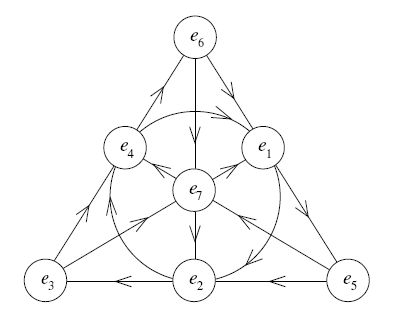
\includegraphics[scale=0.6]{fano}
\centering
\caption{The Fano plane as a mnemonic.}
\end{figure}

\begin{exmp}
The octononions are not asssociative.  For instance 
$$i_0.i_2i_1 = -i_5 $$ $$i_0i_2.i_1 = i_5$$

\end{exmp}
\chapter{Composition algebras}
	One can prove the two-square identity 
	$$	(x_1y_1 - x_2y_2)^2  + (x_1y_2 + x_2y_1)^2 = (x_1 ^{2}+x_2^{2})(y_1 ^{2}+y_2 ^ {2})$$
	
	using the fact that the norm of a product of two complex numbers is the product of the norms. In this section we look into general algebraic structures with this property. We begin with the necessary definitions.
	
	\begin{defn}
		An $ \mathbb{R}-$\textbf{algebra} is a vector space V over the real numbers with a binary operation $ \cdot : V \times V \rightarrow V $ satisfying the following properties:
		\begin{itemize}
		\item Right distributivity: $(x+y) \cdot z = (x \cdot z) + (y \cdot z) $
		\item Left distributivity: $ x \cdot (y+z) = (x \cdot y)+(x \cdot z)$
		\item Compatibility with scalars: $ (ax)\cdot (by) = (ab) (x \cdot y) $
		\end{itemize}
		Here $ x , y \text{ and } z $ denote elements of the vector space while $ a , b $ are elements of the field $ \mathbb{R}. $ A binary operation that satisfies the above three axioms is said to be  \textbf{bilinear}. One need not worry about having separate axioms for right and left distributivity when the binary operation is commutative. However this is not always the case. Indeed, the quaternions are an example of a noncommutative algebra. 
	\end{defn}
	
\begin{exmp}
The set of $ n \times n $ real matrices form an algebra with the usual matrix multiplication.
\end{exmp}
\begin{defn}
	A \textbf{bilinear form} on a vector space V is a bilinear map from $ V \times V \rightarrow F $ where F is the underlying field.
\end{defn} 
\begin{defn}
	A \textbf{degenerate bilinear form} $ f(x,y) $ on a finite dimensional vector space $ V $ is a bilinear form such that it has a non-trivial kernel, i.e., there exists a non-zero $ x $ in $ V $ such that $$ f(x,y) = 0 \; \text{ for all } y \in V.$$
\end{defn}
\begin{defn}
	A bilinear form $ f $ is called \textbf{symmetric} if it satisfies $$ f(v,w) = f(w,v) \; \text{for all } v,w \in V. $$
\end{defn}
\begin{exmp}
The standard dot product on $ \mathbb{R}^n $ is an example of a symmetric bilinear form.
\end{exmp}
\begin{defn}
	A \textbf{nondegenerate bilinear form} on a finite dimensional vector space is a bilinear form that is not degenerate. In other words, $$ f(x,y) = 0 \; \text{ for all } y \in V \text{ implies that } x = 0.$$
\end{defn}
\begin{defn}
	A \textbf{quadratic form} is a map from $ V $ to the underlying field $ F $ satisfying
	\begin{itemize}
		\item $ f(kv) = k^2 v \text{ for all } v \in V \text{ and } k \in F. $
		\item $ b_f(u,v) = f(u+v) - f(u) - f(v) $ is a symmetric bilinear form.
	\end{itemize}
\end{defn}
\begin{theorem}
	If $ f $ is a symmetric bilinear form on $ V, $ then $ f(v) = b_f(v,v) $ is a quadratic form in $ V. $ Furthermore, $ b_f(u,v) = 2 (u,v) \text{ for all } u,v \in V.$
\end{theorem}
\begin{defn}
	A \textbf{composition algebra} over a field $ K $ is a not necessarily associative algebra together with a non degenerate quadratic form N that satisfies $$ N(xy) = N(x)N(y) \; \text{for all } x \text{ and } y \text{ in }A.$$ 
\end{defn}

Throughout this section and the next, we adopt the convention that $ [x]  $ denotes the norm of $ x $ and $ [x,y] $ denotes the inner product of $ x \text{ and } y. $ Here, the inner product $ [x,y] $ is the symmetric bilinear form $ \frac{b_f(u,v)}{2} $ associated with the quadratic from $ [\cdot] $. Hence, we have that $$ [x,y] = \frac{[x+y] - [x] - [y]}{2}.$$ We also assume that our algebra is \textbf{unital}, that is, there exists an identity element satisfying $$ x \cdot 1 = 1 \cdot x =x. $$

\chapter{Properties of composition algebras}
We now explore the properties of composition algebras.
\begin{theorem}
	If $ [x,t] = [y,t] \text{ for all } t $ then $ x = y. $
\end{theorem}
\begin{proof}
	Since $ [x,t] = [y,t], $ we have that $ [x-y,t] = 0 \text{ for all } t. $ Since the norm $ [\cdot] $ is a non-degenerate quadratic form, we must have that $ x-y = 0 $ which gives $ x = y. $
\end{proof}
\section{Multiplication laws}
We state the composition law and deduce its consequences. In the proofs of the theorems that follow, we make considerable use of Theorem 25 and the relation between the inner product and the norm. 
\begin{theorem}
	\textbf{ The Composition Law: }
	\begin{equation}
			[xy] = [x][y] \tag{M1}\label{M1}
	\end{equation}
\end{theorem}
\begin{theorem}
	 \textbf{ The Scaling Laws: }
	 \begin{equation}
	  [xy,xz] = [x][y,z] \tag{M2.1}\label{M2.1} 
	 \end{equation} 
\end{theorem}
\begin{proof}
	Replacing $ y $ by $ y+z $ in  (M1) gives 
	$$ [x(y+z)] = [x][y+z].$$ 
	\begin{align*}
		&&[x(y+z)] &= [xy + xz]\\
		\implies&& [x][y+z] &=[xy]+[xz]+2[xy,xz]\\
		\implies&& [x]([y]+[z]+2[y,z]) &= [xy]+[xz]+2[xy,xz]\\
		\implies&& [x][y] + [x][z] + 2[x][y,z] &= [xy] +[xz]+2[xy,xz]\\
		\implies&& [xy] + [xz] + 2[x][y,z] &= [xy]+[xz]+2[xy,xz]\\
		\implies&& [x][y,z]&=[xy,xz] 
	\end{align*} 
\end{proof}
\begin{equation}
[xz,yz] = [x,y][z] \tag{M2.2}\label{M2.2} 
\end{equation}

 \begin{proof}
 	Replace $ x $ by $ x+z $ in M1. This gives $$[(x+z)y]=[x+z][y] $$
 	\begin{align*}
 			&& [(x+z)y] &= [xy + zy]\\
 			\implies&& [x+z][y] &=[xy]+[zy]+2[xy,zy]\\
 			\implies&& ([x]+[z]+2[x,z])[y] &= [xy]+[zy]+2[xy,zy]\\
 			\implies&& [x][y] + [z][y] + 2[x][y,z] &= [xy] +[zy]+2[xy,zy]\\
 			\implies&& [xy] + [zy] + 2[x][y,z] &= [xy]+[zy]+2[xy,zy]\\
 			\implies&& [x,z][y]&=[xy,zy]  			
 	\end{align*}
 \end{proof}
 \begin{theorem}
 	\textbf{ The Exchange Law: }
 	\begin{equation}
 	[xy,uz] = 2[x,u][y,z] - [xz,uy] \tag{M3}\label{M3}
 	\end{equation}
 \end{theorem}
 \begin{proof}
 	Replacing $ x $ by $ x + u $ in M2.1 gives
 	$$ [(x+u)y,(x+u)z] = [x+u][y,z]$$
 	The left hand side is
 	\begin{align*}
 	[xy+uy,xz+uz] &= [xy,xz]+[xy,uz]+[uy,xz]+[uy,uz]\\
 	&= [x][y,z]+[xy,uz]+[uy,xz]+[u][y,z]\\
 	\end{align*}
 	The right hand side is
 	\begin{align*}
 		[x+u][y,z] &= ([x]+[u]+2[x,u])([y,z])\\
 		&=[x][y,z]+[u][y,z]+2[x,u][y,z]
 	\end{align*}
 	Equating the two sides gives $$ 2[x,u][y,z] = [xy,uz]+[uy,xz] , \text{ as desired.}$$
 \end{proof}
 \subsection{Conjugation Laws}
 \begin{defn}
 The \textbf{conjugate} of $ x $ is defined as $$ \overline{x} = 2[x,1] - x. $$
 \end{defn}
 \begin{theorem}
 	\textbf{ Braid Laws: }
 	\begin{equation}
 	[xy,z] = [y,\bar{x}z] \tag{C1}\label{C1}
 	\end{equation}
 \end{theorem}
 \begin{proof}
  Put $ u = 1 $ in M3. We get 
  \begin{align*}
  [xy,z] &= 2[x,1][y,z] - [y,xz] \\
   &=[y,2[x,1]z]-[y,xz]\\
   &=[y,(2[x,1]-x)z]\\
   &=[y,\overline{x}z]
  \end{align*}
 \end{proof}
 $$ [xy,z] = [x,z\bar{y}]	 $$
 \begin{proof}
 Put $ z =1 $ in M3. We get
\begin{align*}
[xy,u] &= 2[x,u][y,1] - [x,uy]\\
&=[x,u(2[y,1]-y)]\\
&=[x,u\overline{y}]
\end{align*}
 \end{proof}
 \begin{theorem}
 	\textbf{ Biconjugation: }
 	\begin{equation*}
 	\bar{\bar{x}} = x . \tag{C2}\label{C2}
 	 \end{equation*}
 \end{theorem}
 \begin{proof}
 	We use Theorem 25.
 	\begin{align*}
[x,t] = [1.x,t] = [1,\overline{x}t] = [\overline{x}t,1] = [t,\overline{\overline{x}}.1] = [\overline{\overline{x}}.1,t] = [\overline{\overline{x}},t]
	\end{align*}
 \end{proof}
 \begin{theorem}
 	\textbf{ Product conjugation: }
 		\begin{equation*}
 		\overline{xy} = \bar{y}\bar{x} . \tag{C3}\label{C3}
 		\end{equation*}
 \end{theorem}
 \begin{proof}
 	Theorem 25 is used along with (C2).
 	\begin{equation*}
	[\bar{y}\bar{x},t] = [\overline{x} , yt] = [\overline{x}\overline{t},y]  = [\overline{t}, xy] = [\overline{t}.\overline{xy},1] = [\overline{xy},t]	
	\end{equation*}
 \end{proof}
 
  \section{The Doubling Laws}
  \begin{defn}
  Suppose $ H $ is an $ n $-dimensional subalgebra of an algebra $ A $ conatining 1, and $ i $ is a unit vector orthogonal to $ H $. The \textbf{Dickson double} of $ H $ is the algebra $ H+iH $. 
   \end{defn}
   The inner product, conjugation and multiplication on the double of H are given by the following theorems. 
   
  \begin{theorem}
  	\textbf{ Inner-Product Doubling: }
  	\begin{equation*}
  	[a+ib,c+id] = [a,c] + [b,d] \tag{D1}\label{D1}
  	\end{equation*}
  \end{theorem}
  \begin{proof}
  	Since 
  	\begin{align*}
[a,id] = [a\overline{d},i] = 0 \qquad [ib,c] = [i,c\overline{b}] = 0 \qquad [ib,id] = [i][b,d] = [b,d],
  	\end{align*}
  we have $ [a+ib,c+id] = [a,c] + [a,id] + [ib,c] +[ib,id] = [a,c]+[b,d] $.
  \end{proof} 
  \begin{theorem}
  	\textbf{ Conjugation Doubling: }
  	\begin{equation*}
  	\overline{a+ib} = \overline{a} - ib. \tag{D2}\label{D2}
  	\end{equation*}
  \end{theorem}
  \begin{proof}
By definition of conjugate,
\begin{align*}
\overline{a+ib} &= 2[a+ib,1] - (a+ib)\\
&=2[a,1]+2[ib,1] - a - ib\\
&=2[a,1]-a-ib\\
&=\overline{a} - ib.
\end{align*}
  
\end{proof}
\begin{coro}
$ ib = \overline{b}i$.
\end{coro}
\begin{theorem}
	\textbf{ Composition Doubling: }
	\begin{equation*}
	(a+ib)(c+id) = (ac-d\overline{b}) + i(cb + \overline{a}d). \tag{D3}\label{D3}
	\end{equation*}
\end{theorem}
\begin{proof}
Theorem 25 is used again.
	We have the following equalities using previous properties.
	\begin{align}
		&[a.id,t] = [id,\overline{a}t] = 0 - [it,\overline{a}d] = [t,i\overline{a}d] =[i\overline{a}d,t]\\
		&[ib.c,t] = [ib,t\overline{c}] = [\overline{b}i,t\overline{c}] = 0 - [\bar{b}\bar{c},ti] = [\bar{b}\bar{c}.i,t] = [i.cb,t]\\
		&[ib.id,t] = [ib,t.\overline{id}] = -[ib,t.\bar{d}i] = [ib,t.id] \stackrel{\text{M3}}{=} 0 + [i.id,tb] = -[id,i.tb] = -[i][d,tb] = [-d\overline{b},t]
	\end{align}
	Now we use the above to rewrite 
	$$ [(a+ib)(c+id),t] = [ac,t] +[a.id,t] + [ib.c,t]  +[ib.id,t] = [(ac-d\overline{b}) + i(cb + \overline{a}d),t]. $$
\end{proof}
\subsection{Hurwitz's theorem}
The previous subsection and the theorems within constitute a proof of the following theorem.
\begin{theorem}
	If a composition algebra $ Z $ contains a proper subalgebra $ Y, $ it also contains its  double $ Y+iY. $
\end{theorem}

\begin{lemma}
	$ Z = Y + i_Z Y  $ is a composition algebra if and only if $ Y  $ is an associative composition algebra.
\end{lemma}
\begin{proof}
Suppose $ Z = Y + i_Z Y$ is a composition algebra. Then for all $ a, b,c,d \in Y $, we have 
\begin{align*}
&[a+ib][c+id] = [(ac-d\overline{b}) + i(cb + \overline{a}d)].\\
&[a][c]+[a][d]+[b][c]+[b][d] = [ac] - 2[ac,d\overline{b}] + [cb] + 2[cb,\bar{a}d]+[ad].
\end{align*}
Cancelling some terms gives us
$$ [ac,d\overline{b}] = [cb,\overline{a}d] $$
By the braid law,
$$[ac.b,d] = [a.cb,d].$$
Since the above holds for all $ d $ in Y, we have that $ Y $ is an associative composition algebra. The same proof followed in the reverse direction proves the converse.
\end{proof}
\begin{lemma}
	$ Y = X + i_Y X $ is an associative composition algebra if and only if $ X $ is a commutative associative composition algebra.
\end{lemma}
\begin{proof}
Suppose $ Y $ is an associative composition algebra. Then $ X $ must also be an associative composition algebra, by the previous theorem. Since in (5.2) we have shown that $ i_0.bc = i_0c.b $, we can use associativity to obtain $ bc = cb  $ for all $ b,c $ in $ X $. Hence $ X $ is commutative.

For the converse, observe that on expanding out the expressions $ (a+ib).(c+id)(e+if) $ and $ (a+ib)(c+id).(e+if) $ we obtain two expressions that are equal precisely when we use the commutativity and associativity of $ X $.

\end{proof}
\begin{lemma}
	$ X = W + i_X W $ is an associative commutative composition algebra if and only if $ W $ is an associative commutative composition algebra with trivial conjugation.
\end{lemma}
\begin{proof}
	Suppose $ X $ is an associative commutative algebra. Since we have $ ei = i\overline{e} $ by Corollary 1, we use the commutativity of X to get $ e = \overline{e} $ for all $ e \in W. $ Hence $ W $ has trivial conjugation.
	
	Conversely, we need to show that $ X $ is commutative. Note that
	\begin{align*}
	(a+ib)(c+id) = (ac-d\overline{b}) + i(cb + \overline{a}d)\\
	(c+id)(a+ib) = (ca-b\bar{d})+i(ad+\bar{c}d)
	\end{align*}
	are equal exactly when we use the fact that conjugation in $ W $ is trivial along with commutativity.
\end{proof}
We now have all tools to prove the following theorem.
\begin{theorem}
	\textbf{(Hurwitz)}\\ $ \mathbb{R},\; \mathbb{C},\; \mathbb{H},\; \mathbb{O}  $ are the only composition algebras.
\end{theorem}
\begin{proof}
Suppose $ Z $ is an algebra. Since $ Z $ contains $ \mathbb{R} $ as a subalgebra, it must be obtained by repeated doubling of $ \mathbb{R} $ and must the double of some proper subalgebra, unless it is $ \mathbb{R} $ itself. If $ Z $ is $ \mathbb{R}, $ we are done. If not, by Theorem 35, we have that $ Z $ must contain also the double of $ \mathbb{R}, $ which is $ \mathbb{C} $. If now $Z $ is $ \mathbb{C},  $ we are done. Otherwise, $ Z $ must contain the double of $ \mathbb{C} $, which is the quaternions. If $ Z $ is $ \mathbb{H}, $ we are done. Otherwise $ Z$ contains the double of $ \mathbb{H} $ which is the octonions. It seems as though one can repeat this process indefinitely. However we hit a roadblock at the very next step. If $ Z $ is not the octonions, then by Lemma 36, we have that the double of $ \mathbb{O} $ is no longer a composition algebra. Hence we have shown that if $ Z $ is a composition algebra, it must be one of $ \mathbb{R}, \mathbb{C}, \mathbb{H}, \mathbb{O}. $
\end{proof}
\section{Other properties of composition algebras}
\begin{defn}We define the \textbf{inverse} of $ x$ to be 
	$$ x ^ {-1} = \frac{\overline{x} }{[x] } $$
\end{defn}
\begin{theorem}
	\textbf{ Inverse Laws: }
	$$\overline{x}.xy = y = yx.\overline{x}$$
Equivalently, 
	$$x^{-1}.xy = y = yx.x^{-1}$$
\end{theorem}
\begin{proof}
	Theorem 25 and the braid law are used. 
	$$ [\overline{x}.xy,t] = [xy,xt] = [x][y,t] = [[x]y,t].$$
	$$ [yx.\overline{x},t] = [yx,tx] = [y,t][x] = [y[x],t].$$
\end{proof}
\begin{theorem}
	\textbf{ Alternative laws: }
	$$x.xy = x^2 y$$ 
	and 
	$$yx.x = yx^2 $$
\end{theorem}
\begin{proof}
	We use the definition of $ \overline{x} $ in the inverse law (Theorem 40) to get
	$$ (2[x,1]-x).xy = 2[x,1]xy - x.xy  = (2[x,1]-1)x.y = 2[x,1]xy-x^2y.$$
	Cancelling undesired terms gives us the result.
\end{proof}
\begin{theorem}
	\textbf{ Moufang laws: }
	$$xy.zx = x(yz)x = x.(yz)x$$ 
\end{theorem}
\begin{proof}
We have 
\begin{align*}
[xy.zx,t] = [xy,t.\bar{x}\bar{z}]&= 2[x,y][y,\bar{x}\bar{z}] - [x.\bar{x}\bar{z},ty]\\
&=2[x,t][yz,\bar{x}] - [\bar{x}\bar{z}, \bar{x}.ty]\\
&=2[yz,\bar{x}][x,t] - [x][\bar{z}\bar{y},t]\\
&=2[x,\overline{yz}][x,t] - [x][\overline{yz},t]\\
&=[2[x,\overline{yz}]x - [x]\overline{yz} ,t].
\end{align*}
Therefore, $ xy.zx = 2[x,\overline{yz}]x - [x]\overline{yz} $ is a function of $ x$ and $ yz $ only. We can thus replace $ y$ and $ z $ with any two elements such that their product is still $ yz. $ If we replace $ y $ with  $ yz $ and $ z $ with $ 1 $, we obtain $$x(yz).x = xy.zx.$$
On replacing $ y  $ with $ 1  $and $ z $ with $ yz $ we get $$ xy.zx = x.(yz)x$$ 
\end{proof}
\begin{theorem}
		\textbf{ Third alternative law }
		$$xy.x = x.yx $$
\end{theorem}
\begin{proof}
	Replace $ z $ with $ 1 $ in the Moufang Law to get
	$$xy.x = xy.1x = x.(1y)x = x.(y1)x = x.yx $$
\end{proof}
\section{The maps $ L_x $, $ B_x$ and $ R_x $}
The left multiplication, right multiplication, bi-multiplication operators are  defined as:
$$ L_x: y \mapsto xy \qquad R_x: y\mapsto yx \qquad B_x: y \mapsto xyx $$
The third alternative law ensures that the bi-multiplication map is well defined. 
We introduce the notation $$ y^{L_x R_x} := R_x (L_x (y)) $$
$ B_x $ is the product of $ R_x \text{ and } L_x $ without regard to order since 
		$$ y^{L_x R_x} = xy.x = x.yx = y^{R_x L_x} $$
The bi-multiplication map also has a geometric interpretation. Recall the expression for a reflection in the hyperplane perpendicular to a vector $ x $:
$$\text{ref}_x(t) = t - 2\frac{[x,t]}{[x]}x $$ 
Compare this to the expression obtained in the proof of the Moufang laws 
$$xy.zx = 2[x,\overline{yz}]x - [x]\overline{yz} $$
Notice that ref$ _x $ $(\overline{yz} )  = \overline{yz}- 2\frac{[\overline{yz},x]}{[x]}x $. Also,
$ \text{ref}_1(t) = t - 2 \frac{[1,t]}{[1]}1  = -\overline{t}$. Therefore, we have that 
				$$B_x(yz) = xy.zx  = [x](yz)^{\text{ref}_1 \circ \text{ref}_x}$$
	Hence if we take $ z $ to be $ 1 $,we see that $ B_x $ is a scalar multiple of the composition of two reflections.
\section{Coordinates for Quaternions and Octonions}
In this section we recover the usual definition of algebras from the definition using Dickson doubles. We first deal with the quaternions. Let $ i $	be the unit vector that extends $ \mathbb{R} $ to $ \mathbb{C} $ and let $ j $ be the unit vector that extends $ \mathbb{C} \text{ to }\mathbb{H}. $ Note that these unit vectors $ i  \text{ and } j $ are orthogonal to 1 and also each other. We have that $ \text{ref}_1(j) = j $ and $ \text{ref}_i(j) = j $. Hence  $$ iji = B_i(j) = [i]j^{\text{ref}_1 \circ \text{ref}_i} = j$$ We define $ k = ij $.  We thus have $  ki = iji = j $ and $ jk = jij = i.$Also, $ k^2 = (iji)j = j^2 = i(jij) = i^2 $.
We now show $ i^2 = -1 $. Using the braid law, one can write $$[i^2,t] =[i.i,t] = [i,-it] = -[i][1,t] = [-1,t]. $$ We also have that $$ ji = \overline{j}\overline{i} = \overline{ij} = \overline{k} = -k. $$ We have thus obtained the relations 
	
\begin{align*}
		 \qquad &i^2 =j ^2 = k^2 =-1 \\
	        ij &=k \qquad jk =i \qquad ki =j\\
	        ji &= -k \qquad ik = -j \qquad kj = -i 
\end{align*}	

For the octonions, we shall find 7 units $ i_0, \  i_1 \cdots i_6$ such that 
$$\alpha : i_n \mapsto i_{n+1} \text{ and } \beta : i_n \mapsto i_{2n} $$ are symmetries of the multiplication.
$$   $$. The units of the quaternion subalgebra are defined to be 
$$ i_1 = i \qquad i_2 = j \qquad i_4 = k. $$ We let $ i_0 $ be the unit vector which extends $\mathbb{H}  \text{ to } \mathbb{O}. $ Define $ i_0i_n = i_{3n} $. 
Thus we have 
$$ i_0i_1 = i_3 \qquad i_0i_2 = i_6 \qquad i_0i_4=i_5.  $$
Recall that in the proof of Hurwitz's theorem we used the fact that $ i_0.cb = i_0b.c $. We use this to obtain 
\begin{align*}
i_6i_1 = i_0i_2.i_1 = i_0.i_1i_2 = i_0i_4 = i_5\\
i_5i_2 = i_0i_4.i_2 = i_0.i_2i_4 = i_0i_1 = i_3\\
i_3i_4 = i_0i_1.i_4 = i_0.i_4i_1 = i_0i_2 = i_6.
\end{align*}

This shows that each of the 7 triplets $ i_x, i_y, i_z  $ with subscripts 
$$xyz = 124, 235, 346, 450, 561,602, 013 $$ behave like the quaternions. The general such system is $$ i_{n+1}. i_{n+2}, i_{n+4}$$ with $ n $ varying from $ 1 \text{ to } 6. $ This also verifies the assertion that $ \alpha $ and $ \beta $ are symmetries of the multiplication.
\section{Diassociativity}
\begin{theorem}
	The algebra generated by any two octonions is associative.
\end{theorem}	
\chapter{Moufang Loops}	
\section{Inverse loops}
\begin{defn}
	An inverse loop $ L $ is a set with a binary operation, a unary operation the inverse $ \dashv $ and an identity 1 satisfying
	\begin{align}
	x1=1x=x\\
	(x^\dashv)^\dashv = x\\
	x^\dashv. xy =y = yx.x^\dashv
	\end{align}
\end{defn}	
\begin{theorem}
	The inverse of an element $ x $ is unique.
\end{theorem}
\begin{proof}
Suppose $x $ has two inverses $ y $ and $ z $. Then using (6.3)  we get $$ y = y.1 = y.xz = yx.z = 1.z = z. $$
\end{proof}
\begin{theorem}
	In an inverse loop $$(xy)^\dashv = y^\dashv x^\dashv.$$
\end{theorem}
\begin{proof}
	\begin{gather*}
	x^\dashv = x^\dashv.1 = x^\dashv.y^\dashv y = (x^\dashv y^\dashv)y\\
	(x^\dashv y^\dashv)^\dashv x^\dashv = (x^\dashv y^\dashv)^\dashv . (x^\dashv y^\dashv)y =y\\
	(x^\dashv y^\dashv)^\dashv = yx\\
	\text{Taking inverse in the last eqaution above, we get }
	x^\dashv y^\dashv = (yx)^\dashv.
	\end{gather*}
\end{proof}
The relation $ xy=z $ can be written in 6 different ways. This is called a \textbf{hexad} of relations.

\begin{figure}[h]
	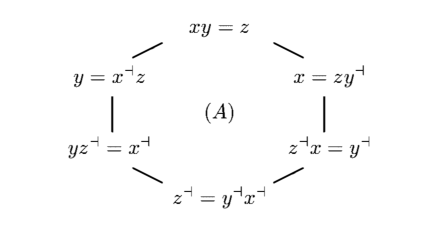
\includegraphics[scale = 0.9]{onqando}
	\centering
	\caption{The duplex form of the hexad.}
\end{figure}

\begin{lemma}
$ yz^\dashv = x^\dashv \Leftrightarrow z^\dashv x = y^\dashv $
\end{lemma}
\begin{proof}
For the  forward direction, note $z^\dashv x =(1.z^\dashv) x = (y^\dashv.yz^\dashv)x = (y^\dashv.x^\dashv)x = y^\dashv$ Conversely, $yz^\dashv  =y(z^\dashv.1) = y(z^\dashv x .x^\dashv) =y (y^\dashv.x^\dashv) = x^\dashv$
\end{proof}
The above equivalence can be rewritten as $ (yz^\dashv)x = 1 \Leftrightarrow y(z^\dashv x) = 1. $ We can then replace $ z $ with $ z^\dashv $ and obtain $ (xy)z = 1 \Leftrightarrow x(yz) =1 $. This makes the parentheses in $ xyz  = 1$ unneccessary. $ xy=z  $ is called the \textbf{duplex} form of the hexad while $ xyz^\dashv =1 $ is called the \textbf{triplex} form of the hexad.
\begin{figure}[h]
	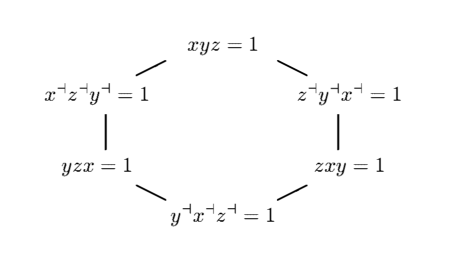
\includegraphics[scale = 0.9]{onqando1}
	\centering
	\caption{The triplex form of the hexad.}
\end{figure}
\section{Isotopy}
\begin{defn}
	An \textbf{isotopy} of a loop $ L $ is a triple of invertible maps that preserve the basic relation $ xy=z $. We introduce two notations for an isotopy according to whether the relation is in duplex or triplex form. By $ (\alpha , \beta | \gamma) $ we mean that $ x^\alpha y^\beta = (xy)^\gamma $. By $ (\alpha ,\beta ,\gamma) $ we mean $ x^\alpha y^\beta z^\gamma = 1.$
\end{defn}
\begin{theorem}
	If $ (\alpha , \beta | \gamma) $ is an isotopy in duplex form, then $ (\alpha ,\beta ,\dashv \gamma \dashv) $ is it's representation in triplex form.
\end{theorem}
\begin{proof}
Suppose $ xyz = 1 $. Then $ xy = z^\dashv$. Applying the isotopy $ (\alpha , \beta | \gamma) $ to this relation, we obtain $ x^{\alpha} y^{\beta} = z^{\dashv\gamma} $. Hence we have that $ x^{\alpha} y^{\beta} z^{\dashv\gamma\dashv} = 1 $. That is, $ (\alpha ,\beta ,\dashv \gamma \dashv) $ is the same isotopy in triplex form.
\end{proof}
\begin{figure}[h]
	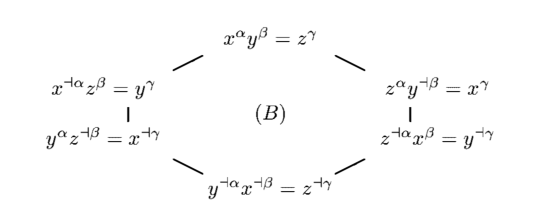
\includegraphics[scale = 0.9]{onqando2}
	\centering
	\caption{On applying $ (\alpha, \beta | \gamma )$ to the basic hexad.}
\end{figure}
If we now rearrange the relations in the above hexad to obtain the $ xy=z $ with variants of the original isotopy applied to it, we obtain

\begin{figure}[h]
	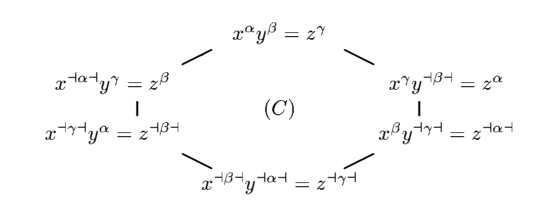
\includegraphics[scale = 0.9]{onqando3}
	\centering
	\caption{Variants of the isotopy $ (\alpha, \beta | \gamma )$}
\end{figure}	
The above two figures represented as a hexad of isotopies in duplex form along with \begin{figure}[h]
	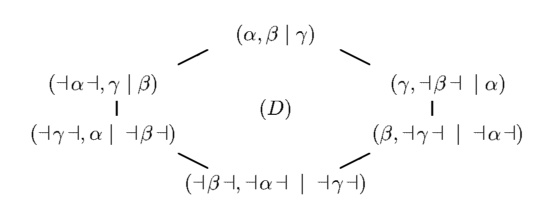
\includegraphics[scale = 0.9]{onqando4}
	\centering
	\caption{Hexad of isotopies in duplex form.}
\end{figure}	
	the same hexad in triplex form after replacing $ \gamma $ with $ \dashv \gamma \dashv $ is shown in Figure 6 and 7.
\begin{figure}[h]
	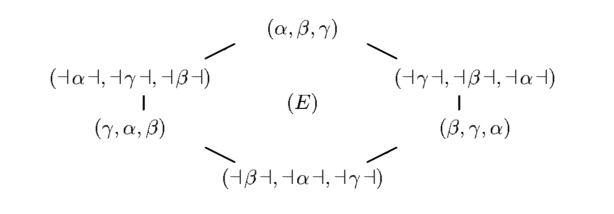
\includegraphics[scale = 0.9]{onqando5}
	\centering
	\caption{Hexad of isotopies in triplex form.}
\end{figure}
\section{Monotopies and companions}
\begin{defn}
	A \textbf{monotopy} is any of the three maps of an isotopy.
\end{defn}
By definition, if $ \gamma $ is a monotopy then there exist maps $ \alpha \text{ and } \beta $ such that $$ xy=z \implies x^\alpha y^\beta = (xy)^\gamma. $$ In particular if we take $ x $ to be $ 1 $ and $ y $ to be $ z $ and then switch $ x $ and $ y $ we obtain  
	$$z^\alpha 1^\beta = z^\gamma , \text{ so } z^\alpha  = z^\gamma 1^{\beta \dashv} = z^\gamma b  $$ 
	$$1^\alpha z^\beta =z^\gamma, \text{ so } z^\beta = 1^{\alpha \dashv}z^\gamma = a z^\gamma. $$

\begin{theorem}
	$ \gamma $ is a monotopy if and only if there are loop elements  $ b $ and $ a $ for which $(xy)^\gamma$ = $ x^\gamma b.ay^\gamma. $
\end{theorem}
\begin{proof}
	The forward direction is a straightforward consequence of the calculation preceding this theorem. For the converse, consider the left and right multiplication operators 
	$$L_a : x \mapsto ax \qquad R_b : x \mapsto bx. $$ Since $(xy)^\gamma$ = $ x^\gamma b.ay^\gamma $ holds, we have that $ (\gamma R_b , \; \gamma L_b |\;  \gamma) $ is an isotopy and hence $ \gamma $ is a monotopy. Here the order of composition in function composition (for instance in $ \gamma R_b $) is to be taken to be opposite of the usual order.
\end{proof}
If such loop elements $ a \text{ and } b  $ exist they are said to be a pair of \textbf{companions} to $ \gamma $. An \textbf{automorphism} is just a monotopy that has $ 1,1 $ as a pair of companions.
\begin{theorem}
	The set of isotopies on an inverse loop $ L $ is a group under the operation defined as 
	$$ (\alpha , \beta, \gamma) \cdot (\alpha', \beta' , \gamma') = (\alpha\alpha', \beta\beta',\gamma\gamma') $$
\end{theorem}
\begin{proof}
Closure is clear since each map in the isotopy is a bijection and the second isotopy applied to $ x^\alpha y^\beta = z^\gamma $ shows that  $ (\alpha\alpha', \beta\beta',\gamma\gamma') $ is an isotopy. Associativity follows from associativity of composition of functions. The identity is the isotopy $ (\mathbbm{1}, \mathbbm{1},\mathbbm{1}). $ The inverse is
$$(\alpha, \beta, \gamma)^{-1} = (\alpha^{-1}, \beta^{-1},\gamma^{-1}) $$
\end{proof}
\begin{lemma}
	$ \dashv L_a \dashv = R_{a^\dashv} $, \qquad $ \dashv R_a \dashv = L_{a^\dashv}  $,\quad $ \dashv B_a \dashv = B_{a^\dashv} $.
\end{lemma}
\begin{proof}
	Observe that using Theorem 46 we have,
	\begin{align*}
	(\dashv L_a \dashv)(x) = (ax^\dashv)^\dashv = xa^\dashv = (R_{a^\dashv})(x)\\
	(\dashv R_a \dashv)(x) = (x^\dashv a)^\dashv = a^\dashv x = L_{a^\dashv}\\
	(\dashv B_a \dashv)(x) = (a x^\dashv a)^\dashv = a^\dashv x a^\dashv  = B_{a^\dashv}
	\end{align*}	
\end{proof}
\begin{theorem}
	If $ a $ is the image of $ 1 $ under some monotopy, then $ L_a, R_{a}, B_{a}, L_{a^\dashv}, B_{a^\dashv}, R_{a^\dashv} $ are monotopies. In particular, if there is any monotopy which takes $ 1 $ to $ a $, then  $ L_a $ and $ R_a $ are such monotopies.
\end{theorem}
\begin{proof}
Consider the product of two isotopies 
$$(\dashv \alpha \dashv , \gamma | \beta)\cdot(\alpha, \beta | \gamma)^{-1} = ( \dashv \alpha \dashv \alpha^{-1} , \gamma \beta^{-1} | \beta \gamma^{-1})$$
Since we have $ \beta \gamma^{-1}  = L_a $ (this is where we use the fact that $ 1 $ maps to $ a $ under some monotopy) and so $ \gamma \beta^{-1} = L_{a^{-1}} $, the product can be rewritten as $$ ( \dashv \alpha \dashv \alpha^{-1} , L_{a^\dashv} | L_a) $$

Applying this isotopy to $ x.a =xa $ gives 
$$a(xa) = x^{\alpha^{-1}\dashv \alpha \dashv}.a^\dashv a = x^{\alpha^{-1}\dashv \alpha \dashv}$$
We can thus identify the map $ \alpha^{-1}\dashv \alpha \dashv $ with the map which takes $ x $ to $ a(xa). $
Thus we have an isotopy which when applied to $ xy=z  $ gives $ a(xa).a^\dashv y = a(xy) $ If we take $ y $ to be $ 1 $ we obtain 
$$ a(xa).a^\dashv = ax, \text{ so } a(xa) = (ax)a$$. This shows that the bimultiplication map $ B_a $ is well defined and that our isotopy is $ ( B_a , L_{a^\dashv} | L_a) $. We obtain the hexad in Figure 6.7 for the isotopy $ (L_a, R_a \;| B_a) $ if we use the following Lemma 51.  

\begin{figure}[h]
	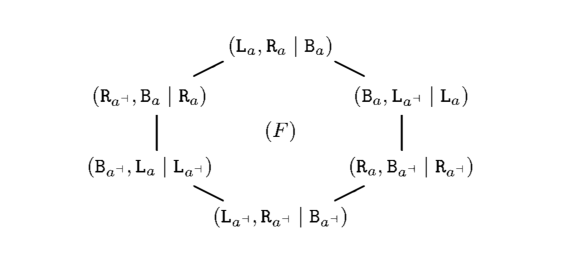
\includegraphics[scale = 0.9]{onqando6}
	\centering
	\caption{Hexad for isotopy $ (L_a, R_a \;| B_a) $ }
\end{figure}

\end{proof}

\begin{theorem}
	The monotopies are transitive if and only if the Moufang identity 
	$$zx.yz = z(xy)z $$ holds.
\end{theorem}
\begin{proof}
	If the monotopies are transitive, there is only 1 orbit of the action of the set of monotopies on the loop. Hence for each element $ z $ in the loop, there is a monotopy $ \alpha $ such that $ \alpha(1) = z. $ By Theorem 52, $ L_z $ is a monotopy and the Moufang identity follows from applying the monotopy $ (L_a, R_a \;| B_a) \text{ to } xy =z$. Conversely, to show that the monotopies are transitive, we show there is only $ 1 $  orbit of the action of monotopies on the loop. That is, every element $ x $ of the loop is the image of a fixed $ y $ under some monotopy. The monotopy we seek is $ L_{xy^\dashv}.  $
\end{proof}
\begin{defn}
A loop for which the Moufang identity holds is called a \textbf{Moufang} loop.
\end{defn}
\begin{exmp}
Every group is an example of a Moufang loop.
\end{exmp}
\begin{exmp}
The nonzero octonions are an example of a nonassociative Moufang loop under octonion multiplication.
\end{exmp}
\section{Different forms of the Moufang Laws}

\begin{theorem}
	We have the three Moufang Laws 
	$$z(xy)z = zx.yz \textbf{ Bi-Moufang Law} $$
	$$z(xy) = zxz.z^\dashv y \textbf{ Left Moufang Law}$$
	$$(xy)z = xz^\dashv .zyz \textbf{ Right Moufang Law}$$
\end{theorem}
\begin{proof}
Using the hexad in (F), we apply the isotopy $ (L_z, R_z \;| B_z) $ to the relation $ xy=z $ to obtain the Bi-Moufang Law $ zx.yz = z(xy)z $. Applying the isotopy $ (B_z, L_{z^\dashv} \; | L_z) $ to $ xy=z $ we get $ zxz.z^\dashv y = z(xy) $. Applying the isotopy $ (R_{z^\dashv}, B_z \; | R_z) $ gives us the Right Moufang Law.
\end{proof}

\hrulefill


	
	
	
	
	
	
	
	
	
	
	
	
	

	



\end{document}
 
 